\chapter{相关技术}
\label{chap:tech}

本系统涉及到了物体追踪、编著与交互系统以及它们之间的通信三部分。物体追踪的实现主要使用了Ren的LibISR工具库\cite{Ren_3DV_2014,star3d_iccv_2013}。为了适配该工具库,需要通过硬件分别获取Kinect的彩色图像和深度图像,进行融合从而获取准确的RGB-D图像,因此需要对使用的Kinect 2进行标定和驱动。标定使用了ROS系统中的Kinect标定工具iai-kinect\cite{iai_kinect2},并且将标定结果进行再加工获得RGB图像与深度图像的映射关系。驱动则使用了开源工具Libfreenect2\cite{libfreenect2}。编著与交互系统基于Unity引擎\cite{Unity}进行了实现,同时使用了Vuforia插件\cite{Vuforia}实现基于增强现实的交互,以及Android SDK\cite{Android}实现移动端的使用。通信则使用了Protocol Buffer\cite{Protobuf, ProtobufNet}串行化数据结构,然后通过TCP通信进行传输。本章将详细介绍上述技术或工具,以及如何将它们应用在本系统当中。

\section{物体追踪相关技术}
\subsection{Kinect驱动}
Kinect是一款微软开发的硬件设备,主要有彩色摄像头,以及红外线发射器和红外线CMOS 摄影机所构成的3D结构光深度感应器。该产品最初被应用于体感游戏,目前则主要被学界用来获取RGB-D图像。本系统使用了Kinect的第二代版本,具有更高的分辨率和性能,但是与第一代相比,他的彩色图像与深度图像分辨率并不成比例,因此在图像使用的过程中需要更多的处理。例如,在进行图像显示的时候,使用相同分辨率的窗口,往往会看到彩色图像和深度图像有不同程度的扭曲。

微软官方提供了Kinect SDK,但是只支持windows系统。此外,还有一些非官方、开源的Kinect驱动。OpenNI\cite{Openni}也提供了开源的对于Kinect传感器的支持,但是目前已经停止更新了,对于Kinect2的支持比较差。此外,还有基于ROS系统的iai kinect\cite{iai_kinect2}可供使用。本系统使用的是libfreenect2\cite{libfreenect2},它基于openni实现,但是对于Kinect2具有比较好的支持。

\subsection{LibISR物体追踪工具}
LibISR是Ren等人基于三维符号距离函数(3D Signed Distance Function )实现的工具库\cite{Ren_3DV_2014, star3d_iccv_2013}。本项目目前只用到了追踪单个物体的部分,这一小节将针对系统中单个物体追踪的算法进行介绍\cite{ren2017real}。

该项目的追踪流程如图\ref{fig:model}所示,首先相机将物体空间下的点映射到相机空间,并且在相机平面成像。该工具在获得相机的RGB-D图像之后,通过前后景分析,将像素分类并反向映射(back-projection)到物体空间,通过他们在物体空间的三维符号函数,得到代价函数,并求出使代价函数局部最小化的解从而还原出物体姿态。

\begin{figure}[!htp]
  \centering
  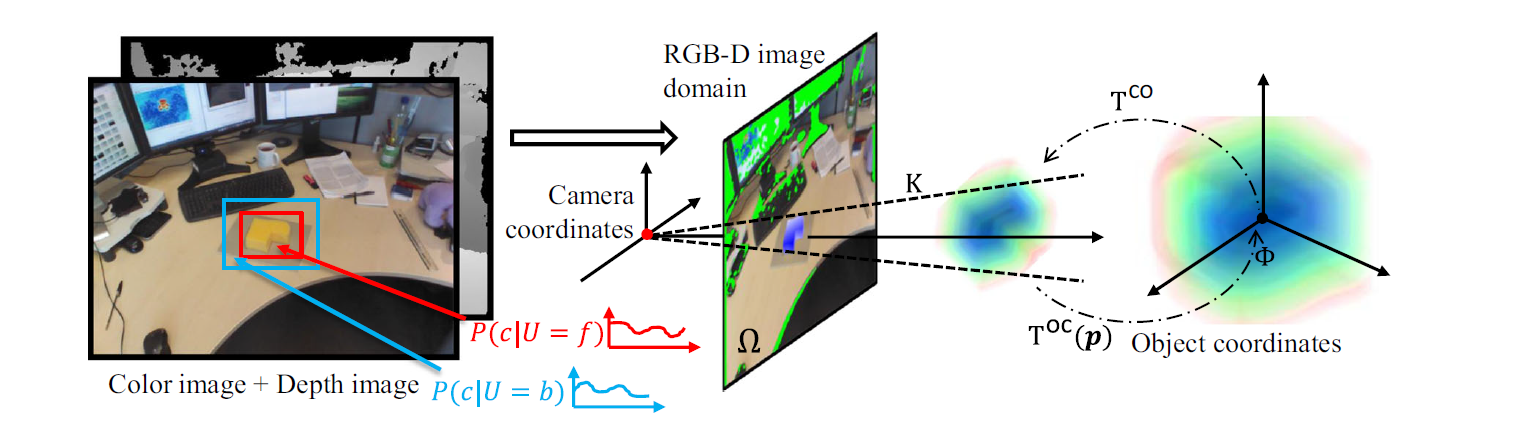
\includegraphics[width=14cm]{figure/model.png}
  \bicaption[LibISR物体追踪流程示意图]
    {LibISR物体追踪流程示意图\cite{ren2017real}}
    {The Flow Diagram of LibISR Tracing Object }
 \label{fig:model}
\end{figure}

LibSIR使用的生成模型(generative model)如图\ref{fig:Gmodel}所示。

\begin{figure}[!htp]
  \centering
  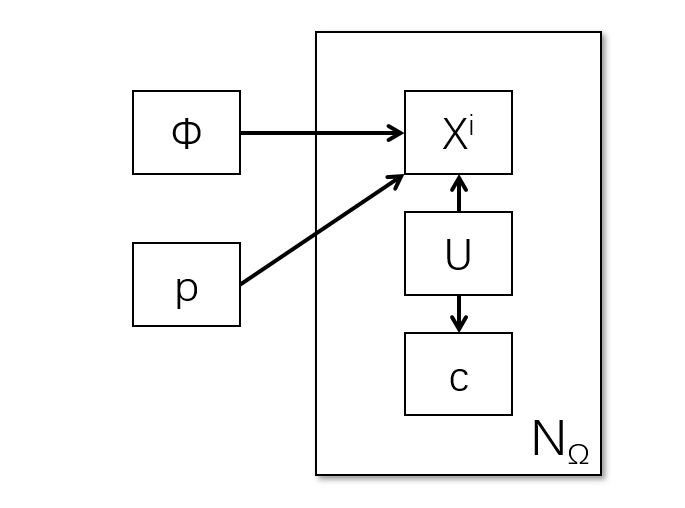
\includegraphics[width=6cm]{figure/jointModel.png}
  \bicaption[LibISR单物体追踪生成模型]
    {LibISR单物体追踪生成模型\cite{ren2017real}}
    {The Generative Model of Tracing Single Object}
 \label{fig:Gmodel}
\end{figure}

其中$p$表示物体的姿态,$\Phi$表示物体的形状。$N_\Omega$表示输入图片中所有像素的集合,$X^i$代表了每个像素的深度值,而$c$代表像素的RGB值。$U$是一个潜变量(latent variable),代表该像素点是前景或后景部分。其中的箭头表示变量之间的依赖关系。

利用上述的生成模型可以估计出联合概率分布(joint probability distribution):
\begin{equation}
 P(X^i, c, U, \Phi, p) = P(\phi)P(p)P(X^i|U, \Phi, p)P(c|U)P(U)\label{L1}
\end{equation}
将公式(\ref{L1})对变量$U$进行边缘化,可以得到公式:
\begin{equation}
 P(X^i, c, \Phi, p) = P(\phi)P(p)\sum_{u\in\{f,b\}}P(X^i|U=u, \Phi, p)P(c|U=u)P(U=u)\label{L2}
\end{equation}

由于图像空间下的坐标点可以通过输入的RGB-D图像以及相机的标定参数反向映射到相机空间,又可以通过物体的姿态信息反向映射到物体空间,因此图像空间的点可以与物体空间的点一一对应,因此可以使用关于物体空间下的函数,即3D SDF函数,描绘图像空间的概率分布。
\begin{equation}
 P(X^i|U=f, \Phi, p)=\delta^{on}(\Phi(X^O))/\eta_f\label{L3}
\end{equation}
\begin{equation}
 P(X^i|U=b, \Phi, p)=H^{out}(\Phi(X^O))/\eta_b\label{L4}
\end{equation}
其中
\begin{equation} \label{L5}
 \delta^{on}(\Phi)=sech^2(\Phi/2\delta) \quad\mathrm{,}\quad
 H^{out}(\Phi)=
 \begin{cases}
    1-\delta^{on}(\Phi) &\Phi\geq0\cr
    0 &\Phi<0
\end{cases}
\end{equation}
\begin{equation}\label{L6}
 \eta_f=\sum_{j=1}^{N_\Omega}\delta^{on}(\Phi(X_j^O))
\quad\mathrm{,}\quad
 \eta_b=\sum_{j=1}^{N_\Omega}H^{out}(\Phi(X_j^O))
\end{equation}
则前后景模型的先验概率可以用公式(\ref{L7})表示
\begin{equation}\label{L7}
 P(U=f)=\eta_f/\eta \quad\mathrm{,}\quad  P(U=b)=\eta_b/\eta \quad\mathrm{,}\quad  \eta=\eta_f+\eta_b
\end{equation}
将公式(\ref{L3}) - (\ref{L7})带入公式(\ref{L2})可以得到对于每一个单独的像素来说,它的联合概率分布为
\begin{equation}\label{L8}
 P(X^i, c, \Phi, p) = P(\phi)P(p)(P(c|U=f)\delta^{on}(\Phi(X^O)) + P(c|U=b)H^{out}(\Phi(X^O)))
\end{equation}

在追踪的时候需要使用RGB-D图像和物体模型数据,通过最大后验概率估计物体姿态。在每个时刻的物体姿态相互独立的基础上,通过条件概率公式可以得到:
\begin{equation}\label{L9}
argmax_{p_t}P(p_t|\Phi,\Omega_t) = argmax_{p_t}\frac{P(p_t,\Phi,\Omega_t)}{P(\Phi,\Omega_t)}
\end{equation}
由于图像中的每个像素都是彼此独立的,因此可以得到
\begin{equation}\label{L10}
P(p_t,\Phi,\Omega_t)=\prod_{j=1}^{N_\Omega}P(X_j^i, c_j, \Phi, p)
\end{equation}
而物体用三维距离函数描绘的物体模型$\Phi$和图像$\Omega$之间也是相互独立的,因此将公式(\ref{L8})和公式(\ref{L10})带入(\ref{L9})可得
\begin{equation}\label{L11}
P(p_t|\Phi,\Omega_t) \sim \prod_{j=1}^{N_\Omega}\Big\{P(c|U=f)\delta^{on}(\Phi(X^O)) + P(c|U=b)H^{out}(\Phi(X^O))\Big\}
\end{equation}
将公式(\ref{L11})求负对数可以得到用于计算的代价函数了
\begin{equation}\label{L12}
\mathscr{E} = -\sum_{j=1}^{N_\Omega}log\Big\{P_j(c|U=f)\delta^{on}(\Phi(X^O)) + P_j(c|U=b)H^{out}(\Phi(X^O))\Big\}
\end{equation}

在最小化该代价函数的过程中,使用了Levenberg–Marquardt算法。该算法通过不断的迭代,搜索出使非线性函数局部最小的数值解。该算法在每一次迭代的过程中计算
\begin{equation}\label{L13}
p^*=\Big\{-[J^TJ + \lambda diag[J^TJ]]^-1\frac{\partial\mathscr{E}}{\partial p^*}\Big\}
\end{equation}
其中$J$是Jacobian矩阵,$\lambda$是算法的惩罚因子,它会在每一次迭代的过程中发生调整。$p^*$是姿态的变化量,通过三维的位移向量和三维旋转向量进行表示。
由公式(\ref{L13}),在每一次迭代之后,将计算出的姿态变化量应用于上一次迭代的姿态结果之上,直到计算出最终的该帧内的姿态变化,并将它应用到上一帧的最终姿态就可以得到物体的变化后的姿态了。
在每次迭代之后,如果将图像空间的点使用姿态信息反向映射到物体空间,会发现具有前景概率大于后景概率的点,会在SDF的影响下不断向物体表面移动,而后景概率较大的点则会不断远离物体,最终得到理想的结果。
由于前后景概率模型对于系统的鲁棒性非常重要,系统会在每帧使用最贴合物体表面,即3D SDF函数值较接近0的点,更新物体的前景概率模型,同时使用目标区域附近的点更新后景模型,以达到更好的效果。其公式为
\begin{equation}
P_t(c|U=u)=(1-p^u)P_{t-1}(c|U) + p^uP_{t-1}(c|U)
\end{equation}
其中$u$为实验得到的参数。

在使用该系统进行物体追踪的过程中,可以发现,单个物体可以在抖动、旋转的过程中仍然具有比较好的追踪效果。但是从本质上讲,使用RGB-D图像对于相机标定的效果,即RGB图像和深度图像的融合效果有比较高的要求,标定的质量很大程度上决定了追踪的效果。此外,受硬件限制,当深度摄像头暴露在强光条件下,也会影响物体追踪的效果。另一方面,从该算法的角度讲,由于物体的姿态、前后景模型都是基于前一次数据累积的,因此当发生追踪错误的时候,追踪误差往往也会累积,影响前后景区分模型,最终很难恢复正确的追踪。

\subsection{CUDA}
上述用于物体追踪的工具LibISR,以及用于驱动Kinect的Libfreenect 2都使用了CUDA\cite{CUDARef}(Compute Unified Device Architecture,统一计算设备架构)进行计算加速。CUDA是由Nvidia公司推出的一套并行计算平台和应用编程接口(API)。用户可以通过CUDA访问GPU的指令集架构(instruction set architecture,ISA),控制显卡中的并行运算模块,提升并发运算速度。由于GPU本身存在很多核心,线程是轻量级的,非常适合进行密集计算任务,例如在图像追踪中就可以用于图像和矩阵的计算。

虽然CUDA基于GPU进行运作,但是实际应用中需要GPU与CPU协同配合。CPU被称为主机端(host),GPU被称为设备端(device)。通常的使用流程是,首先为主机端分配内存,初始化数据。然后将数据复制到设备端,设备端进行运算,运算结束后,将结果复制回主机端,完成任务。GPU中并行执行的函数被称为内核(kernel)。在内核启动GPU进行运算前,必须预先设置GPU的线程结构,包括指定内核的网格(grid)结构,以及每个网格包含的线程块(block)的结构。他们的关系如图\ref{fig:ceda}所示。

\begin{figure}[!htp]
  \centering
  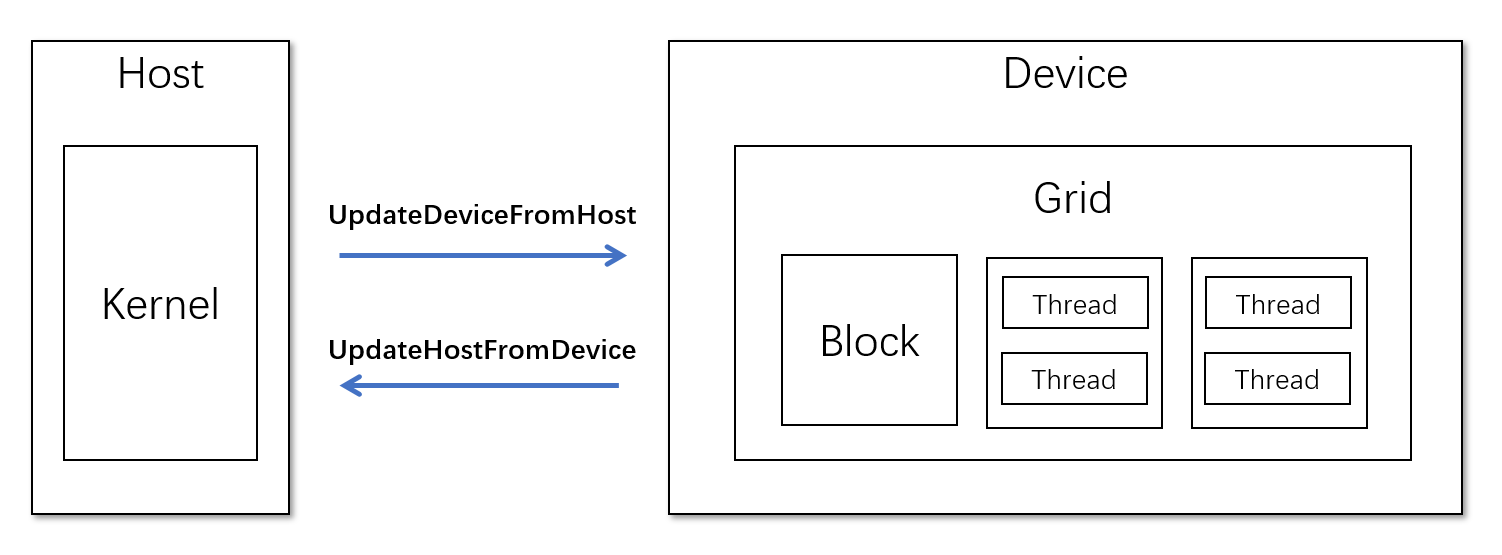
\includegraphics[width=12cm]{cuda.png}
  \bicaption[Kernel上的两层线程组织结构]
    {Kernel上的两层线程组织结构}
    {The Double-Layer Kernel Architecture }
 \label{fig:ceda}
\end{figure}

由图\ref{fig:ceda}可见,通过Block ID和Thread ID就可以唯一的确定一个线程了。而这两个变量也是thread在运行时自己可以直接访问的变量。因此,可以通过它们进行图片或矩阵的遍历和并发。

\section{编著与交互系统相关技术}
面向于教育者的编著系统基于Unity引擎开发,除引擎本身提供的基本功能之外,还使用了Android SDK、Vuforia等插件。本小节将对这些技术进行介绍。

\subsection{Unity引擎}
Unity\cite{Unity}是一款由Unity Technologies开发的引擎。引擎最初是一款针为Mac OS X进行开发的游戏引擎,目前已经扩展至Windows、Android、Play Station、AR、VR等诸多平台,同时仍然保持着轻量级的特点。此外,Unity开发的软件也从最初的游戏,发展为汽车、制造、电影动画、建筑等诸多领域的应用。

Unity项目现在通常基于C\#语言进行开发,以下将对本系统中使用的Unity功能进行介绍。
	
UI方面,Unity提供了按钮、下拉框、文本输出框、选择框等等控件。这些控件可以通过设置画布的自动缩放模式,以及锚点的控制,实现对于不同分辨率的自适应。此外,当这些控件的状态发生变化时,可以触发相应的事件从而控制应用中的游戏对象。除上述控件之外,Unity也可以获取用户的鼠标、键盘事件。对于鼠标的点击事件,在移动端可以自动转换为手指的点击事件,从而减轻了跨平台项目对于代码修改的负担。

游戏控制方面,使用了Game Manager的概念。一般的物体会在应用场景切换的时候被销毁掉,但是Game Manager不会,可以通过它储存信息,并且控制场景切换流程,是一些重要信息在场景切换之后仍然保存。

在基于增强现实交互的过程中,unity会在获得物体的追踪结果之后,在场景中的虚拟物体进行相应的位移、旋转,并最终覆盖在手机的摄像画面上,这是本系统实现增强现实交互的基础。

此外,Unity还提供了控制场景光照、物体材质与着色器、物理模拟与碰撞检测等等功能,都在本项目中有所应用。

\subsection{Android SDK}
Android SDK\cite{Android}是Google开发的提供给Android应用开发人员的软件开发工具包(Software Development Kit,SDK)。对于Unity开发的应用来说,如果需要在Android平台上运行,就需要安装SDK,使Unity可以将项目以Android的架构进行构建(build),以APK的格式发布。

\subsection{Vuforia}
Vuforia\cite{Vuforia}是一款主要基于移动设备,用于实现增强现实应用的软件开发工具包。Vuforia通过摄像头,获得场景图象,然后使用计算机视觉的方法,结合标志物(marker),实现识别、追踪目标物体,最后通过Unity将虚拟物体渲染在手机屏幕的对应位置上。用户通过手机屏幕,就可以看到真实场景与虚拟画面相融合的效果了。
	
对于融合精度要求不高的应用,例如目前市面上多数增强现实游戏,虚拟物体与真实物体并不存在很强的联系。这种情况下,应用往往只需要空间中的任意一点,或是识别出一个可以搭建虚拟场景的平面就可以开始游戏了。一种被广泛应用的增强现实工具是Vuforia Ground Plane\cite{VuforiaGround},用户在开始使用的时候,通过摄像机获取场景信息,然后选定一个理想的平面,虚拟图像就可以以该平面为游戏场景进行绘制了。但是平面识别存在着精度差等问题。当摄像机相对于场景进行移动之后,标记平面的锚点很容易发生偏移,特别是在初始化的平面被摄像头放大、被其他物体遮挡遮挡,或被移出摄像机空间的情况下。

为了提高精度,往往需要在场景或被追踪的物体上添加标志物。目前,Vuforia支持追踪标志物类型包括单张图片(二维码)、立方体、圆柱体或圆台、任意的三维模型四种。用户需要在Vuforia官网获取许可(license),然后使用官网的数据库导入标志物数据,并且在应用中使用对应的许可和数据库,就可以实现相应物体的追踪了。
	
比较常用的是平面标志。平面标志通常由具有一定特征的图片或者二维码组成。Vuforia图片识别的原理是,用户将标志物图片上传后,服务器会将上传的图片转为灰度图,提取其中特征点,打包保存在数据库中。在实时检测的时候,Vuforia会将场景中的图像特征点与数据库中的模板图片特征点数据进行匹配。被用于识别的图片也具有一定的要求,首先需要具有比较高的对比度,而且重复度比较低。被上传到官网的图片的8\%宽度被称为功能排斥缓冲区,该区域并不会被识别。Vuforia还会对上传的图片进行评级,通常带有分明轮廓,棱角分明的图片评级比较高,追踪效果也会比较好。综上所述,二维码非常符合上述条件,所以它本身就是一种非常好的识别标识物。

由于平面标志本身具有位置和尺寸信息,应用可以通过标志物确定出比较准确的物体位置,即使标志物被遮挡或离开相机范围,在标志物返回视野的时候,仍然可以精准的定位。此外,通过计算机视觉识别平面标志的计算效率也比较高。但是平面标志也具有一定的缺点。首先由于平面标志的特性,只有在标志与相机平面平行的时候才有比较好的追踪效果,因此难以追踪可以在三维场景中自由移动的物体。实践证明,当平面标志与相机平面具有一定的倾角的时候,虽然仍然可以识别出倾角,但是可能会发生产生歧义。此外,将平面标志固定在被追踪的物体上,从而保持平面标志与被追踪物体相对静止,往往会影响用户移动物体,而且很容易发生遮挡。因此,平面标志往往被应用于静态的增强现实场景,而很少用于物体追踪。

除了平面标志外,也可以使用三维的标志,如圆柱体,立方体,甚至任意的三维模型等等。通过这些三维标志,物体可以在三维场景中移动时具有比较好的追踪效果,而且可以应对一些遮挡问题。但是,在识别三维标志的时候,相对于平面标志,计算复杂度上升,帧率下降,对于相机性能和拍摄方式的要求也相应提高。被追踪的物体通常不能距离相机太远,而且不能移动过快,因为当物体移动到远处或是快速移动的时候,会在获取的图像中产生模糊影响精度。除此以外,追踪环境的光照对于追踪效果也有比较大的影响。

总的来说,标志虽然能达到比较稳定的追踪效果,但是因为一定的缺陷并不能满足实际需要。除了上述的自身缺陷之外,在使用软件的时候需要用户准备相应的实际标志也是影响标志在实际增强现实软件中难以应用的一个原因。本项目中,出于标定的需要,仅使用了识别效果最好的平面标志作为辅助。

\section{系统间通信相关技术}
\subsection{Protocol Buffer}
Protocol Buffers简称Protobuf,是一种轻便高效的序列化结构数据存储格式,与平台和语言无关,可扩展,因此非常适合用于数据存储和通讯。例如在本系统中,系统前端为基于Unity和C\#语言开发的Android应用,后端是基于C++开发的应用,需要在两者之间跨语言传输信息。如果利用C++ struct定长的特性进行数据序列化和传输,那么不定长的字符串在传输的时候就比较麻烦了。此外,C\#代码需要对接收到的字符串进行解码和赋值,工作量比较大。而且一旦传输对象的结构发生改变,代码修改的负担也比较大。而Protocol Buffers就是一种很方便的结构体数据格式。

在规定协议的时候,需要用户首先设置消息的关键字(message),等同于C\#中的class。关键字包括关键字的名字和消息字段,分别对应C\#总的类名和数据成员。消息字段除了需要规定数据类型,如int32,string等,还需要规定数据的限定符,包括required、optional、repeated三种。Required表示必要数据,optional表示可选数据,repeated表示数组数据。此外,还需要设置不同字段在序列化后的二进制数据中的布局位置。

在使用的时候,只需要将设置好的对象进行初始化,然后序列化编码,发送,接收端接受信息之后反序列化,就可以得到数据了。

\subsection{TCP/IP通信协议}
	TCP(Transmission Control Protocol,传输控制协议)是一种可靠的端到端(host-to-host)的协议。该协议在计算机网络通信的过程中,实现了有序、可查错的信息流(stream)的传输。交换数据的双方被称为一对套接字(socket),由一个IP地址和端口号组成。它是一个抽象概念,当一个程序有了实例化的socket对象,则表示程序被加入到了网络中,可以与网络中的其他应用进行通信。
	
	TCP作为传输层,在计算机网络架构中,处在网络层的上一层。网络层则由IP((Internet Protocol,网际协议)构成。TCP通过IP将变长的数据段发送,由IP进行目的地定位和传输。IP也负责将TCP片段的拆分和整合。由于IP层本身是不可靠的,TCP协议在实现了基本的数据传输的基础上,还负责其他内容。TCP保证了传输数据的可靠性(reliability),即保证数据在重复、乱序、丢失、损坏等情况下的功能恢复。以及流控制(flow control),实现由接收者控制发送者发送的数据量。还有多路复用技术(multiplexing),使单个端可以同时与多个进程进行TCP数据传输。此外,TCP还需要保证连接在创建、数据交换、断开连接的过程中都保证安全。
	
	TCP与IP共同构成了TCP/IP协议族(TCP/IP Protocol Suite),将点对点传输数据的过程中,数据应当如何封装、定位、传输、路由、接受都进行了标准化规定。

\section{本章小结}
综上所述,本章节介绍了系统所使用的技术。首先对比分析了Kinect的各类驱动,之后选择了适合于项目的Libfreenect 2。之后,简要介绍了LibISR中对单个物体追踪的算法,它使用一种基于概率、三维符号函数、代价函数迭代求局部最小值实现物体追踪的算法。之后还简单介绍了硬件加速的工具CUDA的架构。编著系统方面,着重介绍了Unity引擎中使用了的功能,以及其他插件。最后介绍了网络通信协议,包括进行序列化的Protocol Buffers是如何工作的,以及TCP/IP协议。本项目综合使用了上述工具或算法,最终完成了预期需求。